\documentclass[aspectratio=169]{ctexbeamer}
\usepackage{wsnex-beamer}

\title{\textsc{WsNeX} Library Introduction}
\subtitle{Academic \& Technical Manuscript \& Presentation}
\author[SN.WANG]{Shengning Wang \href{mailto:snwang2023@163.com}{\small (snwang2023@163.com)}}
\institute{School of Mechanical Engineering, Dalian University of Technology}
\date{\today}

\begin{document}
% =============================================================================
% 1. TITLE PAGE
% =============================================================================
{
    \usebackgroundtemplate{
        \tikz[overlay, remember picture]\node[opacity=0.6] at (current page.center){
            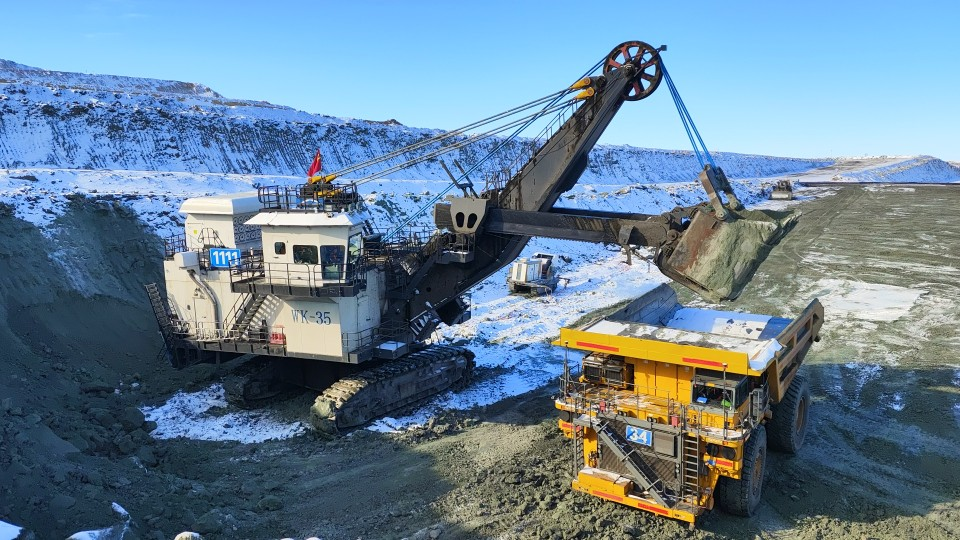
\includegraphics[width=\paperwidth]{fig/BG.jpg}
            };
        }
    \maketitle
}

% =============================================================================
% 2. MAIN BODY
% =============================================================================
\input{}

% example useage
% --- SLIDE 1: Typography & Lists ---
\section{Semantic UI \& Dynamic Lists}
\begin{frame}{\insertsectionhead}
    \begin{itemize}[<+->]
        \item \wsndefi{Semantic Commands}: Use \texttt{\textbackslash \wsnred{wsnred}}, \texttt{\textbackslash \wsnblue{wsnblue}}, or \texttt{\textbackslash \wsndut{wsndut}} for consistent branding.
        \item \wsnalert{Alert System}: The \texttt{\textbackslash \wsnalert{wsnalert}} command highlights critical warnings.
        \item \textbf{Translucent Revelation}:
        \begin{itemize}
            \item Items appear one by one using \texttt{[<+->]} logic.
            \item \onslide<4->{This line is hidden until the 4th click.}
        \end{itemize}
    \end{itemize}
    \wsnfooter{\textsc{WsNeX} adapts to both \wsnalert{Standard Article} and \wsnalert{Beamer} classes.}
\end{frame}

% --- SLIDE 2: Mathematics & Algorithms ---
\section{Advanced Math \& Programming}
\begin{frame}[fragile]{\insertsectionhead}
    \begin{columns}
        \column{0.45\textwidth}
        MLP Architecture:
        \begin{equation}
            \mathbf{h} = \sigma(\mathbf{W}_1 \mathbf{x} + \mathbf{b}_1)
        \end{equation}
        \begin{equation}
            \hat{\mathbf{y}} = ReLU(\mathbf{W}_2 \mathbf{h} + \mathbf{b}_2)
        \end{equation}
        \column{0.55\textwidth}
        \begin{minted}[fontsize=\tiny, bgcolor=lightgray!10]{python}
import torch.nn as nn

class SimpleMLP(nn.Module):
    def __init__(self, in_dim, hid_dim, out_dim):
        super().__init__()
        self.layers = nn.Sequential(
            nn.Linear(in_dim, hid_dim),
            nn.ReLU(),
            nn.Linear(hid_dim, out_dim)
        )

    def forward(self, x):
        return self.layers(x)
        \end{minted}
    \end{columns}
    \wsnfooter{Powered by \texttt{\wsnalert{minted}} and \texttt{\wsnalert{amsmath}} architectures.}
\end{frame}

% --- SLIDE 3: Layouts ---
\section{Geometric Components}
\begin{frame}{\insertsectionhead}
    \begin{block}{Nucleus Architecture}
        The core logic utilizes TikZ for geometric fading and dynamic positioning.
    \end{block}

    \begin{columns}
        \begin{column}{0.5\textwidth}
            \begin{exampleblock}{Geometric Headers}
                Custom frametitle with diagonal joins and automated fading.
            \end{exampleblock}
        \end{column}
        \begin{column}{0.5\textwidth}
            \begin{alertblock}{Global Styling}
                Consistent use of DUT Blue (wsnPrimary) across all UI elements.
            \end{alertblock}
        \end{column}
    \end{columns}
\end{frame}

% =============================================================================
% END COVER
% =============================================================================
{
    \usebackgroundtemplate{
        \tikz[overlay, remember picture]\node[opacity=0.6] at (current page.center){
            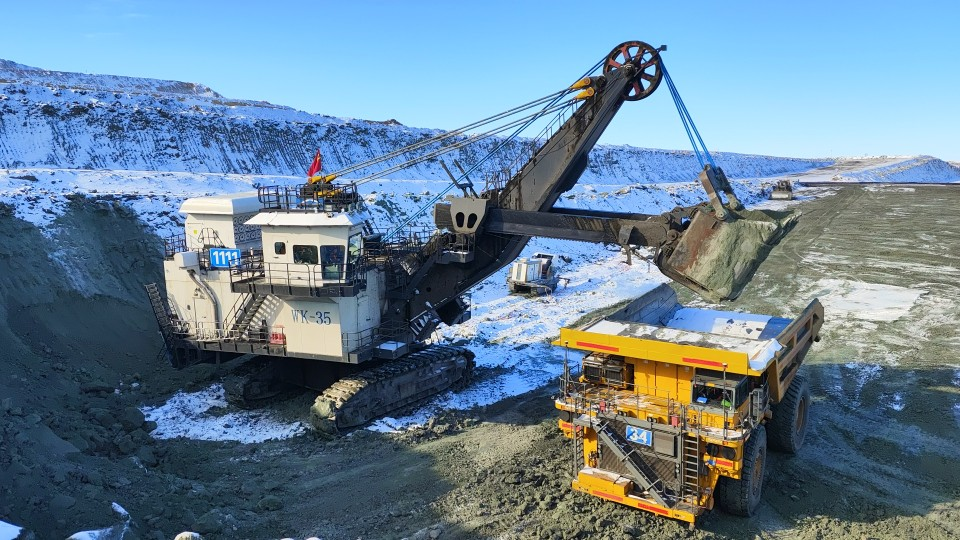
\includegraphics[width=\paperwidth]{fig/BG.jpg}
            };
        }
    \maketitle
}

\end{document}